\documentclass[10pt]{article}
% \usepackage[margin=1in]{geometry}
% \newcommand\hmmax{0}
% \newcommand\bmmax{0}
% % % Fonts% %
\usepackage{luatexja}

\usepackage[T1]{fontenc}
   % \usepackage{textcomp}
   % \usepackage{newtxtext}
   % \renewcommand\rmdefault{Pym} %\usepackage{mathptmx} %\usepackage{times}
\usepackage[complete, subscriptcorrection, slantedGreek, mtpfrak, mtpbb, mtpcal]{mtpro2}
   \usepackage{bm}% Access to bold math symbols
   % \usepackage[onlytext]{MinionPro}
   \usepackage[no-math]{fontspec}
   \defaultfontfeatures{Ligatures=TeX,Numbers={Proportional}}
   \newfontfeature{Microtype}{protrusion=default;expansion=default;}
   \setmainfont[Ligatures=TeX,BoldFont={*-Semibold}]{Source Serif Pro}
   \setsansfont[Microtype,Scale=MatchLowercase,Ligatures=TeX,BoldFont={*-Semibold}]{Source Sans Pro}
   \setmonofont[Scale=0.8]{Atlas Typewriter}
   % \usepackage{selnolig}% For suppressing certain typographic ligatures automatically
% % % % % % %
\usepackage{amsthm}         % (in part) For the defined environments
\usepackage{mathtools}      % Improves  on amsmaths/mtpro2
\usepackage{xfrac}

% % % The bibliography % % %
\usepackage[backend=biber,
  style=authoryear-comp,
  bibstyle=authoryear,
  citestyle=authoryear-comp,
  uniquename=false,
  % allinit,
  % giveninits=true,
  backref=false,
  hyperref=true,
  url=false,
  isbn=false,
  useprefix=true,
  ]{biblatex}
\DeclareFieldFormat{postnote}{#1}
\DeclareFieldFormat{multipostnote}{#1}
% \setlength\bibitemsep{1.5\itemsep}
\newcommand{\noopsort}[1]{}
\addbibresource{Thesis.bib}
% % % % % % % % % % % % % % %

\usepackage[inline]{enumitem}
\setlist[enumerate]{noitemsep}
\setlist[description]{style=unboxed,leftmargin=\parindent,labelindent=\parindent,font=\normalfont\space}
\setlist[itemize]{noitemsep}

% % % Misc packages % % %
\usepackage{setspace}
% \usepackage{refcheck} % Can be used for checking references
% \usepackage{lineno}   % For line numbers
% \usepackage{hyphenat} % For \hyp{} hyphenation command, and general hyphenation stuff

% % % % % % % % % % % % %

% % % Red Math % % %
\usepackage[usenames, dvipsnames]{xcolor}
% \usepackage{everysel}
% \EverySelectfont{\color{black}}
% \everymath{\color{red}}
% \everydisplay{\color{black}}
\definecolor{fuchsia}{HTML}{FE4164}%Neon Fuchsia %{F535AA}%Neon Pink
% % % % % % % % % %

\usepackage[export]{adjustbox}
\usepackage{subcaption}

% \usepackage{pifont}
% \newcommand{\hand}{\ding{43}}
\usepackage{array}

\usepackage{multirow}
% \usepackage{adjustbox}

\usepackage{multicol}

\setcounter{secnumdepth}{4}
\setcounter{tocdepth}{4}

\usepackage{tikz}
\usetikzlibrary{bending,arrows,positioning,calc,arrows.meta,patterns,fadings}
\usetikzlibrary{trees}
\usepackage{tikz-qtree} %for simple tree syntax
% \usetikzlibrary{positioning,shapes.multipart} %for structured nodes
\usetikzlibrary{tikzmark}

\usepackage{graphicx} % for images (png/jpeg etc.)
\usepackage{caption} % for \caption* command

\usepackage{tabularx}

\usepackage{Oblique} % Custom package for oblique commands
\usepackage{CustomTheorems}
\usepackage{FuturePromisedEvents}
\usepackage{ThesisCustom}

% \usepackage{svg}
% \usepackage[off]{svg-extract}
% \svgsetup{clean=true}

\usepackage{dashrule}

\newcommand{\hozline}[0]{%
  \noindent\hdashrule[0.5ex][c]{\textwidth}{.1pt}{}
  %\vspace{-10pt}
  % \noindent\rule{\textwidth}{.1pt}
}

% \usepackage{pdfrender}
\usepackage{extarrows}

% % % My commands % % %

\newcommand{\hozlinedash}[0]{%
  \noindent\hdashrule[0.5ex][c]{\textwidth}{.1pt}{2.5pt}
  %\vspace{-10pt}
}
% % % % % % % % % % % %

\usepackage{xskak} % For chess diagram

\usepackage[hidelinks,breaklinks]{hyperref}

\title{
  Ability to reason and reasoning with ability \\
  \large Outline
}
\author{Ben Sparkes}
% \date{ }

\begin{document}

% \tableofcontents

% \newpage

\maketitle

\section{Interest}
\label{sec:interest}

\subsection{Ability and access to support}
\label{sec:abil-access-supp}

\begin{note}[Introducing main topic]
  Our interest is in when it is permissible for an agent to obtain support for some conclusion of some instance of reasoning on the basis of the support the agent has for the premises of the instances of reasoning.

  We take the following claim as basic:
  \begin{enumerate}[label=\bP{}, ref=\bP{}]
  \item\label{prem:bP} If agent accesses support they have for premises and traces implication through valid and subjectively sound reasoning, then agent obtains support for conclusion on basis of support for premises.
  \end{enumerate}
  For example, suppose an agent has support that one of the three boxes in front of them is red.
  And, the agent has support that the box in front of them has the dimensions of 19 cm x 28 cm x 7cm.
  Some reasoning, the volume of the box is roughly 3,724 cm\(^{3}\).
  Whether some (or all) of the required arithmetic is to be included as a premise may be set aside.
  The support the agent has for holding that the volume of the box is roughly 3,724 cm\(^{3}\) is obtained (at least in part) on the support the agent has for the box having the dimensions noted.
\end{note}

\begin{note}[Support]
  Intuition is, roughly, that agent has support for a proposition if agent has the option of using the proposition in some further reasoning.

  This is not to say that a proposition without support has no use in reasoning.
  
\end{note}

\begin{note}[Valid and subjectively sound]
  Valid and subjectively sound.
  Valid, in the sense that the agent may obtain support for the conclusion.
  In a deductive case, if the premises are true, then the conclusion is true.
  Subjectively sound in the sense that for each premise or step of reasoning used, the agent has support for the premise or step and does not have superior support for a contrary premise or step.
\end{note}

\begin{note}[Focus]
Our interest is with the converse of~\ref{prem:bP}.

\begin{enumerate}[label=\mp{}, ref=\mp{}]
\item\label{denied-claim} An agent obtains support for conclusion on basis of support the agent has for premises only if the agent accesses support they have for premises and traces implication through valid and subjectively sound reasoning.
\end{enumerate}
If the agent did not measure the box, nor perform the arithmetic, the agent would not obtain support.
A luck guess that the box is roughly 3,724 cm\(^{3}\) would not allow the agent to hold that the volume of the box is roughly 3,724 cm\(^{3}\) on the basis of the dimensions of the box.
\end{note}

\begin{note}[Alternative]
  Our interest with \ref{denied-claim} is that it is a universal claim --- \ref{denied-claim} applies to all instances in which an agent obtains support for conclusion on basis of support for premises.

  Our goal is to motivate an exception to \ref{denied-claim}.

  \begin{enumerate}[label=\rC{}, ref=\rC{}]
  \item\label{rC} If an agent has information that they have the ability to (soundly) reason to some conclusion, then the agent may obtain support for the conclusion on basis of support for premises that the agent would access by witnessing their ability to reason to the conclusion.
  \end{enumerate}

  \ref{rC} carves an exception to~\ref{denied-claim}.
  For, if~\ref{rC} is true, then there are cases in which an agent is not required to reason from premises to some conclusion in order to obtain support for the conclusion on the basis the support the agent has for the premises.
\end{note}

\begin{note}[Structure of argument]
  Two lines of argument for endorsing~\ref{rC}, and hence denying~\ref{denied-claim}.
  \begin{enumerate}[label=(L\arabic*), ref=(L\arabic*)]
  \item\label{arg:line:1} Motivate~\ref{rC} as resolution to tension resulting from~\ref{denied-claim}.\newline
    Specifically:
    \begin{enumerate}[label=(L1\alph*)]
    \item\label{arg:line:1:a} Provide recipe for generating scenarios where~\ref{denied-claim} is in tension with particular scenarios involving information that an agent has the ability to perform some reasoning and a further claim regarding support.
    \item\label{arg:line:1:b} Motivate~\ref{rC} as a resolution to the tension.
    \end{enumerate}
  \item\label{arg:line:2} Argue that granting~\ref{rC} as an exception to~\ref{denied-claim} allows for an intuitive understanding of cases in which agent has the option of appealing to ability, even if there are alternative ways of interpreting the scenario in line with~\ref{denied-claim}.
  \end{enumerate}
  These two lines of argument work together.
  The tension of~\ref{arg:line:1} generates interest in witnessing that may be flatly rejected by prior endorsement of~\ref{denied-claim}.
  The intuitive understanding of scenarios involving ability of~\ref{arg:line:2} suggests there's more to witnessing than resolving the tension in narrow cases.
\end{note}

\begin{note}[Details of \ref{arg:line:1}]
  The initial focus is on the first line of argument,~\ref{arg:line:1}.
  The tension developed in part~\ref{arg:line:1:a} is delicate, but hopefully informative.
  We will establish a number of corollaries regarding ability and the interaction between~\ref{denied-claim} and ability.
\end{note}

\begin{note}[Before turning to the argument\dots]
  Before turning to the argument, we conclude this introduction with a handful of notes regarding~\ref{denied-claim} and~\ref{rC}.
\end{note}

\begin{note}[Interest in ability]
  Idealised agents have no need to appeal to ability.
  However, for limited agents, ability is abundant, while the resources required to witness abilities are scarce.
  That the exception to~\ref{denied-claim} is narrow does not entail that there are few occurrences of the exception.

  Information about ability may be abundant while the resources for witnessing abilities are either scarce or temporarily unavailable.
  So, agent is able to conserve or defer use of resources.

  Broadening scope.
  Arguments involving~\ref{denied-claim}.
  Distinction between ideal and non-ideal.
  Potential alternative conclusions to arguments that appeal to~\ref{denied-claim} as a premise.
  Revise premises for arguments in which~\ref{denied-claim} is a conclusion.
\end{note}

\begin{note}[Scope of \mp{}]
  \mp{} does not say anything in particular about what the agent has support for, only what must be the case in order for an agent to appeal to support for some conclusion on the basis of support for premises.

  Talking in terms of (support for) premises and conclusions restricts attention to reasoning.
  There may be broader use of `premise' and `conclusion' where an agent is not required to reason from premise to conclusion in order for the premise to support the conclusion.
  For example, if visual perception is immediate.
  Perhaps it may be said that an agent's visual experience is a premise to the conclusion that a dog is sleeping.
  Still, for present purposes, `conclusion' refers to the output of some process of reasoning performed by an agent which is either actual or potential, and `premises' to the input of that process.

  Note, also, that in both cases the relation between premises and conclusion is important.
  If agent does not reason, then neither~\ref{prem:bP} nor~\ref{denied-claim} apply.
  If there are multiple ways to obtain a conclusion, then~\ref{denied-claim} does not require the agent to reason from a particular set of premises.

  Likewise,~\ref{denied-claim} does not require that an agent is required to obtain support for a proposition by valid and subjectively sound reasoning from some premises.

  Rather,~\ref{denied-claim} requires that an agent reason from premises to conclusion in order to establishes support between premises and conclusion
  By contrast,~\ref{prem:bP} holds that reasoning is sufficient to establish such a relation.
\end{note}

\begin{note}[\mp{} is intuitive]
  \ref{denied-claim} is intuitive, and is quite common, though not without exceptions.
(For example, there's views on testimony in which the testifier provides agent access to support the testifier has.
One may understand this as conflicting with~\ref{denied-claim}, or that the fact that these are accessible is the relevant piece of support.)
\end{note}

\begin{note}[Alternative]
  \ref{rC} restricts~\ref{denied-claim}.
  This is not to say the agent obtains support equivalent to that which would be obtained were the agent to do, or have done, the reasoning.
  Nor, that the agent is aware of the relevant premises.

  Intuitively, \rC{} states that the agent may appeal to the reasoning they are able to perform in support for the conclusion of that reasoning, and as that reasoning moves from premises to conclusion, it is on the basis of the support for those premises that the agent would identify by reasoning that the agent obtains (some) support for the conclusion.

  Hence, \rC{} is in line with the spirit of~\ref{prem:bP}.
  For the exception to~\ref{denied-claim} is granted by the agent appealing to a witnessing event in which the antecedent (and consequent) of~\ref{prem:bP} are satisfied.
\end{note}

\begin{note}[Doxastic (as opposed to propositional) support]
  This is `doxastic' as opposed to `propositional'.
  Agent need not reason in order to have propositional support.
  For example, \(A < B\) and \(B < C\), then propositional support for \(A < C\) even if I don't bother to reason.
  No further assumptions about the relation between propositional and doxastic support.
\end{note}

\begin{note}[Ability ensures propositional?]
  Plausible that if the agent has the ability, then the agent already has propositional support for the relevant proposition.
\end{note}

\subsection{Broad argument overview}
\label{sec:broad-argum-overv}

\begin{note}[Overview]
  Tension resulting from the unrestricted scope of~\ref{denied-claim}.
  We begin by introducing a particular type of scenario involving ability, and observe how~\ref{denied-claim} requires a unique interpretation of the scenario.
  We then introduce an additional principle regarding support, which conflicts with the interpretation of the type of scenario introduction required by~\ref{denied-claim}.
\end{note}

\subsection{Type of scenario}
\label{sec:type-scenario}

\begin{note}[Tension, information]
  The tension arises when an agent is provided with a piece of limited information that:
  \begin{enumerate}[label=(I\arabic*), ref=(I\arabic*)]
  \item So long as the agent has a general ability, then the agent has a specific ability.
  \end{enumerate}
  The information is limited because it does not directly provide the agent with the information that the agent has the specific ability, nor that the result of witnessing the specific ability is the case.

  For example,
  \begin{enumerate}[label=(I\arabic*), ref=(I\arabic*), resume]
  \item\label{qe:cond} So long as you have the ability to reason with the rules of chess, you have the ability to demonstrating that there is a sequences of moves that will ensure a win for one of the players (as an instance of the general ability).
  \end{enumerate}
  The conditional structure distinguishes this information from:
  \begin{enumerate}[label=(I\arabic*), ref=(I\arabic*), resume]
  \item\label{qe:cons} You have the ability to demonstrate that there is a sequences of moves that will ensure a win for one of the players.
  \end{enumerate}
  For the agent is required to obtain~\ref{qe:cons} from~\ref{qe:cond}.
  In turn, the agent is not provided with information that:
  \begin{enumerate}[label=(I\arabic*), ref=(I\arabic*), resume]
  \item\label{qe:result} There is a sequences of moves that will ensure a win for one of the players.
  \end{enumerate}
  For, it need not be the case that~\ref{qe:result} is true if~\ref{qe:cond} is true by virtue of a false antecedent.
  Of course, the antecedent of~\ref{qe:cond} need not be false.
  Still, the limited information requires the agent to appeal to their general ability in order to obtain information about how the agent's general ability extends to a particular case.

  However, if the agent hold that they have the ability to demonstrate that there is a sequences of moves that will ensure a win for one of the players, then the agent may reason to~\ref{qe:result}.

  \begin{enumerate}
  \item[\textsf{A}]\label{A:s} On the one had, a strategy must exist in order for the agent to possess the ability to demonstrate that a strategy exists.
  \item[\textsf{W}]\label{W:s} On the other hand, if the agent has the ability to demonstrate that a strategy exists, then there it is possible for the agent to witness an event in which they demonstrate that a strategy exists.
  \end{enumerate}
  We term these \AR{} and \WR{}, respectively.

  We will return to this kind of limited information in greater detail below.
  For now, the basic idea is that the agent is on the hook, so to speak, for holding that they have the specific ability.
  Perhaps the informer does not want the agent to rely on the informer's information for the existence of the strategy.
  Or, perhaps the agent only wants to appeal to their own understanding of chess.

  We don't need a fleshed out scenario, but if it helps,~\ref{qe:cond} may be read as a slight challenge.
  The relevant interpretation of `if you're smart enough, you can solve this problem' seems clear.
  `If your ability to reason is of sufficient worth, then by extension of that ability, you have the ability to solve this problem.'
  Paraphrased, `if you're smart enough, you have the ability to solve this problem'.
  So challenged, and confident in one's smarts, one may expect to solve the problem.
  The slight difference with the limited information of interest is that the informer provides information about what the solution to the problem is if the agent is `smart enough'.
\end{note}

\begin{note}[Scenario premise]
  For ease of reference, we wrap scenarios involving the limited information as a premise.
  \begin{enumerate}[label=\eA{}, ref=\eA{}]
  \item\label{prem:ab} It is possible for an agent to use information that they have some specific ability so long as the agent has some general ability to obtain support for what follows from the specific ability.
    (Where the agent lacks doxastic support for what follows, and for \(A(\psi)\) without information).
  \end{enumerate}
\end{note}

\begin{note}[Attribute]
  There is not yet tension between~\ref{denied-claim} and~\ref{prem:ab}.
  For, we noted that the agent may appeal to their ability to reason in either of two ways:
  \begin{enumerate}[label=\(\cdot\)]
  \item \AR{}: \(\phi\) must be the case in order to have the attribute of being able to reason to \(\phi\).
  \item \WR{}: There is a (potential) witnessing event in which \(\phi\) is demonstrated, and therefore \(\phi\) is the case.
  \end{enumerate}
  WR{} is an instance of~\ref{rC}, as the agent obtains support for the conclusion of the reasoning is able to do on the basis of the reasoning that would be performed in a witnessing event.
  Hence, the supported obtained for the conclusion is obtained on the basis of the support the agent has for the premises that would be used.
  Again, this does not imply that the agent obtains support for the conclusion which is equivalent to the support the agent would obtain by witnessing their ability by performing the reasoning.

  However, \AR{} suggests an alternative way to obtain support for the conclusion of reasoning the agent is able to do.
  Specifically, if order for the agent to \emph{have} the attribute of being able to reason to the conclusion, the conclusion of the reasoning must be true.
  The relevant inference is in part secured by the verb chosen, and in part by what the verb is applied to.
  Here, `demonstrate' is a factive verb, if an agent demonstrates that \(\phi\), then it is true that \(\phi\).
  And, the existence of a chess strategy does not depend on the agent demonstrating that the relevant strategy exists.

  To take another example, you only have the ability to identify a typo on this page if there is a typo on this page.
  So, if I were to provide you with testimony that you have the ability to identify a typo on this page, you may begin searching for the typo, or you may note that there must be a typo in order for me to be in a position to provide you with testimony that you have the ability.

  The reasoning is summarised with the following sketch.

  \begin{enumerate}[label=(\textsf{A}\arabic*), ref=(\textsf{A}\arabic*)]
  \item\label{WR:Sketch:1} I have the attribute of being able to \emph{V} that \(\phi\).
  \item\label{WR:Sketch:2} In order to have the attribute of being able to \emph{V} that \(\phi\), \(\phi\) must be the case independent of whether or not I witness the ability.
  \item\label{WR:Sketch:3} \(\phi\) is the case.
  \end{enumerate}

  To keep things simple, we will refer to the principle behind the pattern sketched as \AR{}.
  And agent may bundle~\ref{WR:Sketch:1} and~\ref{WR:Sketch:3} into a conditional, and avoid instantiating the reasoning pattern, but so long as the conditional is (implicitly) held on the basis of the intermediate premise~\ref{WR:Sketch:2}, we take use of such a conditional to be an instance of \AR{}.

  \AR{} is compatible with \ref{denied-claim}.
  For, the two premises~\ref{WR:Sketch:1} and~\ref{WR:Sketch:2} are accessible to the agent, and obtaining \ref{WR:Sketch:3} from~\ref{WR:Sketch:1} and~\ref{WR:Sketch:2} appears to be straightforwardly sound reasoning.
\end{note}

\begin{note}[Established conditional 1]
  We wrap the above observations in a conditional.
  \begin{enumerate}[label=(C\arabic*), ref=(C\arabic*)]
  \item\label{P:ab-and-dc:W} If
    \begin{enumerate}[label=(C1\alph*), ref=(C1\alph*)]
    \item an agent obtains support for some proposition \(\phi\) on the basis of the agent's ability to demonstrate that \(\phi\) is the case, and
    \item \ref{denied-claim} is true,
    \end{enumerate}
    then the support for \(\phi\) is obtained on the basis of the agent having the attribute of being able to demonstrate that \(\phi\) (in line with \AR{}).
  \end{enumerate}
\end{note}

\begin{note}[Broader conditional]
  For present purposes,~\ref{P:ab-and-dc:W} is our focus.
  Still, the observations made when establishing~\ref{P:ab-and-dc:W} broader relation between \ref{denied-claim} and ability.
  For, we noted that \ref{denied-claim} is incompatible with \WR{}.
  To recap:
  \begin{enumerate}[label=(B\arabic*), ref=(B\arabic*)]
  \item Assume an agent appeals to entailment from the ability to \emph{V} that \(\phi\) in order to obtain \(\phi\).
  \item The agent makes use of (the reasoning sketched in) either \AR{} or \WR{}.
  \item \WR{} is incompatible with~\ref{denied-claim}.
  \item The agent makes use of (the reasoning sketched in) \AR{}.
  \end{enumerate}
\end{note}

\subsection{Additional principle}
\label{sec:additional-principle}

\begin{note}[Finding tension, still]
  At present,~\ref{P:ab-and-dc:W} (merely) establishes that~\ref{P:ab-and-dc:W} constrains how an agent may use information about reasoning they are able to do.
  There is of yet no explicit tension.

  Still, given that~\ref{P:ab-and-dc:W} requires the agent to obtains support in a specific way (\AR{}), we turn to whether it is permissible for the agent to obtain support in the context of~\ref{prem:ab}.
\end{note}

\begin{note}[Inertia]
  Our final main premise is:\nolinebreak
  \footnote{
    A few caveats may be required here.
  }
  \begin{enumerate}[label=\nI{}, ref=\nI{}]
  \item\label{prem:ni} An agent does not have the option of obtaining support for some proposition \(\psi\) on the basis of information that the support the agent has for \(\phi\) is misleading or mistaken if \(\psi\) is not the case.
  \end{enumerate}

  The key idea is that in order for support to go through, the agent needs to be clear on how the support the agent has for \(\phi\) is also support for \(\psi\).

  {
    \color{red}
    A slightly better way of putting things for my purposes is that \(\phi\) does not inherit support from \(\psi\).
    So, \(\phi\) may be supported, but no support is added.
  }

  {
    \color{red}
    The agent may obtain support for \(\phi\) from some other premise.
  }

  For example, explanatory connexion.

  % A restricted instance of \ref{prem:ni} is entailed by cases of misleading evidence about evidence.
  % Here, the higher-order support is misleading else the lower order support is misleading.
  % The agent has a problem, for sure.
  % Still, \ref{prem:ni} does not entail (a restricted instance) of misleading higher order evidence.
  % For,~\ref{prem:ni} constraints only how an agent's support may be applied --- it is compatible with there being no higher order support.

  I consider \ref{prem:ni} to be intuitive.
  However, argument may be provided.
\end{note}

\begin{note}[Some motivation for \ref{prem:ni}, 1]
  Some motivation for~\ref{prem:ni} may be found by constructing instances of reasoning which violate~\ref{prem:ni}.
  A couple of cases may help.

  For example, suppose our agent is out shopping for a gift for Sam with a friend and has not yet considered the items before them.
  The friend remarks that `Someone would only buy \emph{that} (some particular item) as a gift for Sam if they didn't know Sam very well.'
  The agent has support that they do know Sam very well.
  However, it does not seem permissible for the agent to obtains support that they wouldn't buy that as a gift, one the basis of the support they have their familiarity with Sam and the statement made by their friend.
  For, it is possible that they agent would have settled on the particular item if they had given it some consideration --- the support the agent has for their familiarity with Sam \emph{may} be misleading.

  Or, suppose the agent has parked their car on the street outside of Sam's place and reasons that:
  If my car is stolen then my support that this is a safe neighbourhood would be misleading.
  Therefore, as my support that this is a safe neighbourhood is not misleading, my car has not been stolen.
  The agent's reasoning seems confused.
  Perhaps the agent has the option of extending the support the have that the neighbourhood is safe to obtain support that they car remains parked outside, but that support the agent has would be misleading if their car has been stolen does not seem appropriate.
\end{note}

\begin{note}[Some motivation for \ref{prem:ni}, 2]
  For further motivation, consider undercutting defeaters.

  We take the following sketch from \textcite{Worsnip:2018aa}:
  \begin{quote}
    Undercutting defeaters, which are easiest to think of in the context of the attitude of belief, are supposed to be considerations that undermine the justification of a belief in a proposition p not necessarily by providing (sufficient) positive evidence to think that p is false, but rather merely by suggesting (perhaps misleadingly) that one’s reasons for believing p are no good, in a way that neutralizes or mitigates their justificatory or evidential force.\nolinebreak
    \mbox{}\hfill\mbox{(\citeyear[29]{Worsnip:2018aa})}
  \end{quote}

  Undercutting defeaters are of interest with respect to~\ref{prem:ni} is that (merely) suggesting that the agent's support for \(\phi\) is no good can amount to highlighting that the agent's support for \(\phi\) may be misleading.

  Consider the following illustration provided by \citeauthor{Pollock:1987un}\nolinebreak
  \footnote{
    \citeauthor{Pollock:1987un} defines an undercutting defeater as follows:
    \begin{quote}
      R is an \emph{undercutting defeater} for P as a prima facie reason for S to believe Q if and only if
      \begin{enumerate}[label=(UD\arabic*), ref=(UD\arabic*)]
      \item P is a reason for S to believe Q and R is logically consistent with P but (P and R) is not a reason for S to believe Q, and
      \item R is a reason for denying that P wouldn't be true unless Q were true.\nolinebreak
        \mbox{}\hfill\mbox{(\citeyear[485]{Pollock:1987un})}
      \end{enumerate}
    \end{quote}
    Intuitively, an undercutting defeater for P as a reason for Q because it the defeater denies that Q must be true in order for P to be true.
  }\nolinebreak
  :
  \begin{quote}
    [Undercutting defeaters] attack the connection between the reason and the conclusion rather than attacking the conclusion itself.
    For instance, ``X looks red to me'' is a prima facie reason for me to believe that X is red.
    Suppose I discover that X is illuminated by red lights and illumination by red lights often makes things look red when they are not.
    This is a defeater, but it is not a reason for denying that X is red (red things look red in red light too).
    Instead, this is a reason for denying that X wouldn't look red to me unless it were red.\nolinebreak
    \mbox{}\hfill\mbox{(\citeyear[485]{Pollock:1987un})}
  \end{quote}
  Completing \citeauthor{Pollock:1987un}'s example, it seems that if agent's support for holding that X is red is that `X wouldn't look red to me unless it were red', then the support for X being red provided by appearance is retracted after discovering that X is illuminated by red lights (though it remains possible that X is red).

  Assumption --- in violation of \ref{prem:ni} --- an agent always has the option to obtain support for \(\psi\) on the basis of information that the support the agent has for \(\phi\) is misleading if \(\psi\) is not the case.

  Given that it remains possible that X is red, it follows that the appearance of X being red would be misleading if X is not red.
  For, it continues to be the case that X appears to be red, even after the discovery is made by the agent.
  Therefore, by the assumption violating~\ref{prem:ni}, support for X being red persists in the presence of the undercutting defeater.
  Still, intuitively it seems that the undercutting defeater of a red light blocks the agent obtaining support for X being red on the basis of their visual perception.

  This is partial motivation for~\ref{prem:ni}, as substituted `does not have the option' from the text of~\ref{prem:ni} with `always has the option' when making the problematic assumption.
  Further argument is (hopefully) to follow.
\end{note}

\begin{note}[Inertia and attribution]
  \ref{prem:ni} raises a problem for applying \AR{} to the specific ability of scenarios described by~\ref{prem:ab}.

  For, the agent is required to obtain specific ability from general ability.
  \begin{enumerate}
  \item Agent has support for the general ability to reason with the rules of chess.
  \item However, the agent has not demonstrated the existence of the strategy, and so the agent relies on the information provided by the informer to hold that they have the specific ability to demonstrate the existence of the strategy.
  \item Still, the informer provided by the informer requires the agent to endorse having the general ability to reason with the rules of chess.
  \item In turn, that whatever support the agent has for having the general ability to reason with the rules of chess is not misleading.
  \item For, it may be the case that the agent does not have the ability to demonstrate the existence of the particular strategy.
  \item Therefore, the agent does not obtain support for the ability to demonstrate the existence of the strategy.
  \item Hence, it is not an option for the agent to obtain support for the existence of the strategy on the basis of support for the ability to demonstrate the strategy in line with \AR{}
  \end{enumerate}
\end{note}

\begin{note}[Established conditional 2]
  We wrap the above observations in a conditional.
  \begin{enumerate}[label=(C\arabic*), ref=(C\arabic*)]
    \setcounter{enumi}{1}
  \item\label{P:ab-and-dc:A} If
    \begin{enumerate}[label=(C2\alph*), ref=(C2\alph*)]
    \item an agent obtains support for some proposition \(\phi\) on the basis of the agent's ability to demonstrate that \(\phi\) is the case, and
    \item \ref{prem:ab} is true,
    \end{enumerate}
    then the support for \(\phi\) \emph{may not be} obtained (in line with \AR{}) on the basis of the agent having the attribute of being able to demonstrate that \(\phi\).
  \end{enumerate}
\end{note}

\begin{note}[Established conditional 2]
  Something about, if \ref{prem:ab} then agent does not obtain support for the attribute.
\end{note}

\begin{note}[Summary]
  Given the two established conditionals~\ref{P:ab-and-dc:W} and~\ref{P:ab-and-dc:A}, the combination of the key premises of \ref{denied-claim},~\ref{prem:ab}, and~\ref{prem:ni} are in tension.

  For, combining~\ref{P:ab-and-dc:W} and~\ref{P:ab-and-dc:A} we have:
  \begin{enumerate}[label=(CC), ref=(CC)]
  \item If \ref{prem:ab} is the case an agent obtains support for some proposition \(\phi\) on the basis of the agent's ability to demonstrate that \(\phi\) is the case then:
    \begin{enumerate}[label=(C\arabic*\(\sim\)), ]
    \item If \ref{denied-claim} is true, then the support for \(\phi\) is obtained on the basis of the agent having the attribute of being able to demonstrate that \(\phi\) (in line with \AR{}).
    \item If \ref{prem:ni} is true, then the support for \(\phi\) \emph{may not be} obtained (in line with \AR{}) on the basis of the agent having the attribute of being able to demonstrate that \(\phi\).
    \end{enumerate}
  \end{enumerate}
  In short, if~\ref{prem:ab} is the case then~\ref{denied-claim} requires a certain interpretation of the scenarios identified by~\ref{prem:ab} and~\ref{prem:ni} denies that the interpretation is plausible.
\end{note}

\begin{note}[Tension, choices]
  The combination of~\ref{P:ab-and-dc:W} and~\ref{P:ab-and-dc:A} is complex.
  However, the basic structure is straightforward:
  \[\ref{prem:ab} \rightarrow ((\ref{denied-claim} \rightarrow \AR{}) \land (\ref{prem:ni} \rightarrow \lnot \AR{}))\]
  Rewriting:
  \[\ref{prem:ab} \rightarrow ((\lnot \AR{} \rightarrow \lnot \ref{denied-claim}) \land (\AR{} \rightarrow \lnot \ref{prem:ni}))\]
  Hence:
    \[\ref{prem:ab} \rightarrow ((\WR{} \rightarrow \lnot \ref{denied-claim}) \land (\AR{} \rightarrow \lnot \ref{prem:ni}))\]
  Simplifying:
  \[\ref{prem:ab} \rightarrow ((\WR{} \land \lnot \ref{denied-claim}) \lor (\AR{} \land \lnot \ref{prem:ni}))\]
  A reformulating as a distinction:
  \[\lnot \ref{prem:ab} \lor (\WR{} \land \lnot \ref{denied-claim}) \lor (\AR{} \land\lnot \ref{prem:ni})\]

  In short, we have the following resolutions.
  \begin{enumerate}
  \item\label{ten:res:nS} Agent may not obtain support for result of witnessing ability, or
  \item\label{ten:res:nD} Agent obtains support for result on the basis on premises that the agent would use when witnessing ability --- incompatible with general application of~\ref{denied-claim}
  \item\label{ten:res:nI} Agent obtains support for result from attribute of having the ability on the basis that the support they have for general ability would be misleading --- incompatible with general application of~\ref{prem:ni}
  \end{enumerate}
  \ref{ten:res:nS} is incompatible with~\ref{ten:res:nD} and~\ref{ten:res:nI}.
  However, \ref{ten:res:nI} and~\ref{ten:res:nD} are compatible, as both~\ref{denied-claim} and~\ref{prem:ni} may be restricted.
\end{note}

\begin{note}[Argument sketch recap]
  Let us recap the main points of the argument so far.
  \begin{enumerate}
  \item Assume possibility of cases in which agent is provided with information that they have some specific ability so long as the agent has a general ability, such that the agent has support for having the general ability, but has not established support for possessing the specific ability.
  \item In such cases, it seems it is possible for the agent to obtain support for what follows from the agent witnessing their specific ability.
  \item If so, the agent appeals to having the specific ability in order to obtain support for what follows from the agent witnessing their specific ability.
  \item Attribution, and witnessing.
  \item If witnessing, then conflict with the requirement that an agent must access support for the premises appealed to in support of a conclusion.
  \item If attribution, then conflict with the restriction that an agent may not obtain support for some proposition on the basis that support the agent has for some other proposition would be misleading otherwise.
  \end{enumerate}

  To follow:
  \begin{enumerate}
  \item Restricting~\ref{denied-claim} in favour of~\ref{rC} works well.
  \end{enumerate}
\end{note}

\begin{note}[Meek outlook]
  This is not a clean argument.
  Take~\ref{denied-claim} and~\ref{prem:ni} and hold the first.
  The agent may not obtain support.

  While there may be tension if the agent obtains support, this tension is never instantiated.

  I am sympathetic.

  Still, endorsing the restriction does not require the agent to obtain support in this case.
  Harbour some hope that that there is scope to restrict \ref{denied-claim}, and that the argument provided for resolving tension in favour of \rC{}, along with later arguments, may serve as a source for reflection.
\end{note}

% \begin{note}[Next steps]
%   The plan is as follows:
%   \begin{enumerate}
%   \item Introduce an example case.
%   \item Develop tension.
%   \item Introduce principle.
%   \item Sketch argument.
%   \item Work through details of the argument.
%   \end{enumerate}
% \end{note}

\newpage

\section{Tension}
\label{sec:tension}

\subsection{Type of case}
\label{sec:type-case}

\subsubsection{Chess}
\label{sec:chess}

\begin{note}[Information]
\begin{enumerate}
\item\label{chess:claim:1}\label{chess:claim:1:conditional} If you are able to reason with the rules of chess, then you have the ability to demonstrate that White cannot prevent Black from occupying c4 on their (Black's) second move given the game state (described in figure~\ref{fig:chess:board}).
\end{enumerate}
\end{note}


\begin{figure}[h]
  \centering
  \mbox{ }
  \hfill
  \begin{subfigure}{.4\textwidth}
    \begin{adjustbox}{minipage=\linewidth,scale=0.7}
      \centering
      \newchessgame[
      setwhite={ka5,pa3,pb4,pc4,pe5,pf6,bg5,bh5}, %{rc1,kh1,pa2,pb2,ph2,pf6,pg6,nc7,qf7},
      addblack={pa6,pb7,pc6,pe6,pf7,kc7,nd7,nd4}, %{rg2,pb5,pe5,qd6,pa7,pb7,ra8,bc8,kd8,bf8},
      ]%
      \setchessboard{showmover=false}%
      \chessboard
    \end{adjustbox}
    \caption{
      Game state\newline
      \mbox{ }\newline
    }
    \label{fig:chess:board}
  \end{subfigure}
  \mbox{ }
  \hfill
  \mbox{ }
  \begin{subfigure}{.4\textwidth}
    \begin{adjustbox}{minipage=\linewidth,scale=0.7}
      \centering
      \newchessgame[
      setwhite={ka5,pa3,pb4,pc4,pe5,pf6,bg5,bh5}, %{rc1,kh1,pa2,pb2,ph2,pf6,pg6,nc7,qf7},
      addblack={pa6,pb7,pc6,pe6,pf7,kc7,nd7,nd4}, %{rg2,pb5,pe5,qd6,pa7,pb7,ra8,bc8,kd8,bf8},
      ]%
      \setchessboard{showmover=false}%
      \chessboard[
      arrow=latex,
      linewidth=1pt,
      shortenstart=.8ex,
      shortenend=.5ex,
      pgfstyle=straightmove,
      strokeopacity=0.4,
      fillopacity=0.4,
      color=black,
      pgfstyle=border,
      markfields={c4,a3,a5,g6,c5},
      % markmoves={b7-b6,c6-c5,d4-c2,d4-b5,d4-f5,d4-e2,d4-f3,d4-b3,d7-c5,d7-b6,d7-b8,d7-f8,d7-f6,d7-e5,d7-e5,c7-c8,c7-b8,c7-d8,c7-b6,c7-d6}%{f7-g8,f7-e6,f7-d5,f7-c4,f7-b3,f7-e8,c7-d5,c7-b5,c7-a8,c7-e8,g6-g7,a2-a3,b2-b3,c1-a1,c1-b1,c1-d1,c1-e1,c1-f1,c1-g1,h2-h3,h1-g1,c1-c2,c1-c3,c1-c4,c1-c5,c1-c6}
      ]
    \end{adjustbox}
    \caption{Example fields White cannot prevent Black from occupying after two moves.}
    \label{fig:chess:move}
  \end{subfigure}
  \hfill
  \mbox{ }
  \caption{Black to checkmate in four moves.\protect\footnotemark}
  \label{fig:chess}
\end{figure}
\footnotetext{
  \citeauthor{Emms:2000aa}' Puzzle 150 (\citeyear[33]{Emms:2000aa}).
  \citeauthor{Emms:2000aa} provides the following solution:
  \begin{quote}
    \variation{1... Nb6!}
    (threatening \variation{2... Nb3\#})
    \variation{2. b5}
    (or \variation{2. Bd1 Nxc4+} \variation{3. Ka4 b5\#})
    \variation{2... c5!}
    \variation{3. bxa6 Nxc4+}
    \variation{4. Ka4 b5\#}
    \textbf{(0-1)}\nolinebreak
    \mbox{}
    \hfill
    (\citeyear[46]{Emms:2000aa})
  \end{quote}
}

\begin{note}[Role of conditional]
  Claim~\ref{chess:claim:1} is distinct from the claim that the agent has the ability to demonstrate a strategy --- the unembedded consequent of claim~\ref{chess:claim:1}
\begin{enumerate}
\item\label{chess:claim:2}\label{chess:claim:1:conditional} You are able to reason from the game state (described in figure~\ref{fig:chess:board}) to the proposition that White cannot prevent Black from occupying c4 on their (Black's) second move.
\end{enumerate}
\end{note}

\begin{note}[Reasoning sketch]
  With the above, sketch out simple reasoning.
  \begin{enumerate}[label=(S\arabic*), ref=(S\arabic*)]
  \item\label{inf:cond:ant} I have the ability to reason with the rules of chess.
  \item\label{inf:cond} If I have the ability to reason with the rules of chess then I have the ability to demonstrate the existence of a (particular) strategy.
  \end{enumerate}

  As~\ref{inf:cond:ant} is the antecedent of~\ref{inf:cond} and the consequent of~\ref{inf:cond} is novel information,~\ref{inf:cond:ant} and~\ref{inf:cond} combine to provide support for:

  \begin{enumerate}[resume, label=(S\arabic*), ref=(S\arabic*)]
  \item\label{inf:cond:conq} I have the ability to demonstrate the existence of the (particular) strategy that White cannot prevent Black from occupying c4 on their second move.
  \end{enumerate}

  Note, however, that~\ref{inf:cond:conq} is not considered a straightforward application of \emph{modus ponens}.
  Rather,~\ref{inf:cond} captures conditional information about how some ability the agent has extends, if it is indeed the ability to reason with the rules of chess.

  Sub-conclusion~\ref{inf:cond:conq}, is the antecedent of the following quantified conditional:

  \begin{enumerate}[resume, label=(S\arabic*), ref=(S\arabic*)]
  \item\label{inf:gae} For any strategy, an agent has the ability to demonstrate the existence of the strategy only if the strategy exists.
  \end{enumerate}

  Therefore:

  \begin{enumerate}[resume, label=(S\arabic*), ref=(S\arabic*)]
  \item\label{inf:sse} The (particular) strategy (that I am able to demonstrate) exists.\newline
    White cannot prevent Black from occupying c4 on their second move.
  \end{enumerate}
\end{note}

\begin{note}[How premise applies to argument]
  \ref{denied-claim} is a universal claim.
  Applies to all instances of reasoning.
  So, trace the support for general ability and information to the conclusion.
\end{note}

\subsubsection{Additional sketches}
\label{sec:additional-sketches}


\section{Attrubtion and Witnessing}
\label{sec:attr-witn}

\begin{note}[Overview]
  In this section we examine the type of ability statements used in some detail.

  \begin{itemize}
  \item The potentive inference.
  \item \AR{} and \WR{}.
  \item Differences between \AR{} and \WR{}.
  \item (Possibly) further notes on \WR{}.
  \end{itemize}
\end{note}

\subsubsection{Potentive entailment}
\label{sec:potentive-entailment}

{
  \color{red}
  Replace `inference' with `entailment', as I don't want to focus solely on the use of this in reasoning.
}

\begin{note}[Overview]
  We being with a general overview of the potentive inference.
  After establishing the basics, we then turn to the two ways outlined.
  \AR{} and \WR{}.
\end{note}

\begin{note}[Potentive inference]
  In order for there to be potential that \(\phi\) is the case, \(\psi\) must be the case.

  Potentive = adjective of potential.
\end{note}

\begin{note}[Examples]
  Simple instances of the potentive inference involve factive verbs, in which the relevant fact holds independently of whether the verb is witnessed.
  \begin{itemize}
  \item Sam has the ability to show that \(19\) is a prime number.
  \item Taylor has the ability to derive Transposition.
  \item Jesse has the ability to \dots
  \end{itemize}

  Note also that the verb does not need to involve some reasoning.
  \begin{itemize}
  \item Corey has the ability to see there is a zebra in the pen.
  \item X has the ability to hear that there is a waterfall nearby.
  \end{itemize}
\end{note}

\begin{note}[Breaking things down]
  \begin{quote}
    \emph{S} has the ability to \emph{V} that \(\phi\).
  \end{quote}
  We have
  \begin{itemize}
  \item Some result of the verb.
  \item A verb.
  \item Modal, ability.
  \item Copula.
  \item An agent.
  \end{itemize}
  As noted, potentive inference works because certain things must be the case in order for there to be a potential event.
\end{note}

\begin{note}[Understanding of the inference]
  The key parts of the inference are the relation between ability and the verb.

  Certain things must be true in order for the verb.
  These are the things which are obtained by the potentive inference.

  In the case of reasoning, note that there must be premises from which the agent works from.
\end{note}

\begin{note}[Observation in terms of propositional/doxastic]
  One way to view this is that if the agent has information, then the agent may infer that they have propositional support for the conclusion which may be turned in to doxastic support.
\end{note}

\begin{note}[Some formal stuff]
  \[\exists e(\text{Able}(s,e) \land (V(e) \land \text{agent} = s \land \text{result}(e) = \phi))\]
  There is some event \(e\), such that \emph{s} is able to bring about, and \(e\) consists of \emph{s} \emph{V}ing with the result that \(\phi\).

  This requires some non-standard existential, but we're not too interested in providing an analysis suitable for semantics.

  Still, there's nothing too special about the position of the existential.
  Understand ability as relating the agent directly to an event.
  Alternative it to take a truth value.
  \((\text{Able}(s,\exists (V(e) \land \text{agent} = s \land \text{result}(e) = \phi))\).

  Close to having a possible world with \(\phi\) and accessibility relation.
  Interpret the non-standard existential in this way, if it helps.
  There is some possible world and some event in that world, such that the agent at the world of evaluation is able to perform the event witnessed at the possible world.

  In both cases, it's the role of the event.

  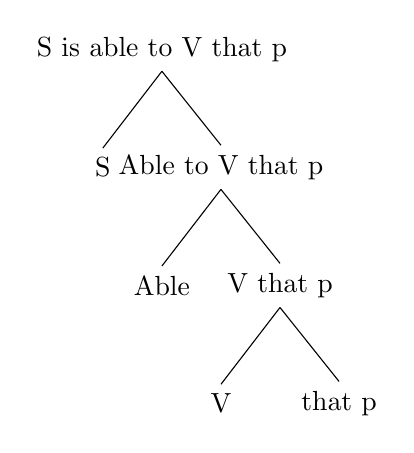
\begin{tikzpicture}[
    ]
    \node{S is able to V that p}
    child {node {S}}
    child {node {Able to V that p}
      child {node {Able}}
      child {node {V that p}
        child {node {V}
        }
        child {node {that p}
        }
      }
    };
  \end{tikzpicture}

  Take some arbitrary witnessing event.
  If \(\psi\) follows from the (arbitrary) witnessing event, then we have an instance of the potentive inference.
\end{note}

\begin{note}[Expanding the event]
  The description of the witnessing event given is minimal.
  Still, simply add in more detail as desired.
\end{note}

\begin{note}[Specific abilities]
  Applies to specific abilities, as the inference appeals to a witnessing event.
  Analogue holds with respect to general abilities.

  General example:
  \begin{itemize}
  \item Sam has the ability to reason with the rules of chess.
  \end{itemize}
  Infer that there is a body of rules governing chess.
  If there are no rules governing chess, then the agent does not have the ability to reason with those (non-existing) rules.

  Not an instance of the potentive inference, as this doesn't follow from what is required from a witnessing event.

  Similarly, it may be that there is an entailment from general to specific.
  \begin{itemize}
  \item If general, then specific.
  \end{itemize}
  For example, understand the general ability distributively.
  Again, not an instance of the potentive inference, as this doesn't follow from what is required from a witnessing event.
\end{note}

\begin{note}[Paraphrasing (footnote)]
  Various paraphrases are available.
  \begin{itemize}
  \item Corey can see there is a zebra in the pen.
  \end{itemize}
  `Can' introduces the complexity that the agent may be witnessing.
  For example, we observe an excited look appear on Corey's face as they look into the pen.
  `Ah, Corey can see a zebra in the pen.'
  Corey isn't exited because they have the ability to see a zebra in the pen, rather Corey is excited because they are seeing a zebra.
\end{note}

\begin{note}[Restriction on instances of the potentive inference]
  We're interested in certain examples as the agent has all of the resources required, so to speak.

  To illustrate, place the reasoning examples behind a conditional.
  \begin{itemize}
  \item If you teach Sam \dots [factoring method], then Sam will have the ability to show that \(19\) is a prime number.
  \end{itemize}
  Intuitively, this is the result of assuming that some additional property holds of the agent.
  Hence, \(\alpha(s) \rightarrow \dots\).
  For, \(\alpha(s)\) will allow the attribution of ability to be true.
\end{note}

\begin{note}[Reasoning and premises]
  Important to note is that in cases of reasoning, the potentive inference may be applied to obtain the availability of premises.

  The difference is the role of these premises.
\end{note}

\begin{note}[Moving on to a more detailed understanding]
  How exactly the event works.
\end{note}

\subsubsection{\AR{} and \WR{}}
\label{sec:ar-wr}

\begin{note}[Overview]
  Interest is in how potentive entailment is used.

  A clearer understanding of \AR{} and \WR{}.

  The significant difference is with reasoning.
  \AR{} uses (a variation of) the potentive inference to obtain support.
  \WR{} uses information obtained by the potentive inference to obtain support.
\end{note}

\begin{note}[Diagram]
  \begin{figure}[h]
  \begin{subfigure}{.5\textwidth}
    \centering
    \begin{tikzpicture}[
      ->,
      >=stealth',
      % auto,
      node distance=0cm, every text node part/.style={align=center},
      ]

      \node [] (c) at (0,0) {};
      \node [] (d) at (-3,0) {};
      \node [] (e) at (3,0) {};
      \node [] (f) at (0,-2.1) {};

      \node (1) at (0,-.1) {Ability};
      \node (2) at (0,-2) {Conclusion};

      \draw [->] (1.270) to [] node[left] {} (2.90);
    \end{tikzpicture}
    \caption{\AR{}}
    \label{fig:AR:support}
  \end{subfigure}
  % \hfill
  \begin{subfigure}{.5\textwidth}
    \centering
    \begin{tikzpicture}[
      ->,
      >=stealth',
  % auto,
      node distance=0cm, every text node part/.style={align=center},
      ]

      \node [] (c) at (0,0) {};
      \node [] (d) at (-3,0) {};
      \node [] (e) at (3,0) {};
      \node [] (f) at (0,-2.1) {};

      \node (premise) at (0,-.1) {Premise};
      \node (conclusion) at (0,-2) {Conclusion};

      \node (x) at (-2,-1.05) {Ability};
      \draw [->] (1.270) to node[left] (3) {} (2.90);

      \node (4) [left of=3, xshift=-2cm] {}; % {\(\exists f (f\Phi = \psi)\)};
      \draw [-{Circle[open]}, dashed] (x.0) to (premise);
      \draw [-{Circle[open]}, dashed] (x.0) to (conclusion);

    \end{tikzpicture}
    \caption{\WR{}}
    \label{fig:WR:support}
  \end{subfigure}
  \caption{Relations of support for \AR{} and \WR{}}
  \label{fig:ARandWR:support}
\end{figure}
\end{note}

\begin{note}[Examples of support relation]
  The interesting issue is the inaccessibility of the premises.
  However, there are other examples in which the same structure is present, but premises are accessible.
  
  Are there other instances of information being used in this way?

  Plausible that go from appearance to support.

  `You are looking at a dog'.

  Here, the agent can infer from testimony that the animal is a dog.
  On the other hand, the agent can take the information to establish a support relation.
  So, visual perception support that the animal is a dog.

  Or, a little better.
  These are coyote tracks.
  Then, different ways to support presence of coyote.
  One is the information provided.
  The other is the tracks.
\end{note}

\begin{note}[The event]
  Two ways for the potentive inference to function.
  Both \AR{} and \WR{} focus on the witnessing event.

  \emph{V}ing that \(\phi\).
  \begin{itemize}
  \item \(\phi\) must be the case in order for the agent to \emph{V} that \(\phi\).
  \item In order for the agent to have the attribute \dots
  \item \(\phi\) is the result of the agent \emph{V}ing.
  \item As a result of witnessing the ability \dots
  \end{itemize}

  So, \AR{} doesn't consider the relevant witnessing, only what must be the case in order for there to be a witnessing event.
  By contrast, \WR{} focuses on guarantees about what transpires in the witnessing event.
\end{note}

\subsubsection{\AR{}}
\label{sec:ar}



\subsubsection{\WR{}}
\label{sec:wr}

\begin{note}[Overview]
  Understanding \WR{}.
\end{note}

\begin{note}[Work backwards for the event]
  
\end{note}



\begin{note}[How support works]
  In the case of reasoning, the result will be that the agent has information about premises.
  Here, it is important to note that the agent has `propositional' support for the premises, independent of the ability information.
  So, the agent does not need to appeal to the existence of the event as a premise in obtaining support for the conclusion.
  The only relevant support the agent has is the support for the premises.
\end{note}




\subsubsection{Distinction between \AR{} and \WR{}}
\label{sec:dist-betw-ar}

\begin{note}[Overview]
  The important difference is what supports the conclusion.

  Here, we suggest that further differences depend on additional commitments.
\end{note}


\begin{note}[Key Issue]
  The key issue is whether the agent obtains support for all the relevant preconditions of witnessing the ability by witnessing.
  And, whatever follows from this, e.g.\ in terms of commitments and so on.

  If so, then anything that follows from \AR{} also follows from \WR{}.
  Conversely, as the agent does not obtain information about how the ability is witnessed, it seems what follows from \WR{} also follows from \AR{}.
\end{note}

\begin{note}[Interesting case]
  Interesting case to think about, in which the agent obtains support for what follows from witnessing, but intuitively not for some other precondition.
  \begin{itemize}
  \item Ability to reason to \(\phi\).
  \end{itemize}
  Inference applies to \(\phi\).
  Inference doesn't seem to apply to reasoning to \(\lnot\phi\) as mistaken.
\end{note}

Understanding of ability is such that there is always a potential witnessing event.

\ref{denied-claim} and~\ref{prem:ni} are universal claims.
\ref{prem:ab} is an existential claim.
\ref{denied-claim} and~\ref{prem:ni} clash in scenarios where the possibility captured in~\ref{prem:ab} is realised.

The collection of~\ref{denied-claim},~\ref{prem:ni}, and~\ref{prem:ab} is in tension.

There is an additional secondary premise:

\begin{note}[Two ways to understand ability and support]
\begin{enumerate}
\item\label{prem:ability} Two ways to obtain conclusion given ability.
  \begin{enumerate}
  \item Attribution.
  \item Witnessing.
  \end{enumerate}
\end{enumerate}

\ref{prem:ability} does not make a claim about any particular use of ability.
As a template, conceptually (or logically) coherent.
If there's a problem, then it's because there are further constraints on understanding of support.
\end{note}


\subsection{Inertia}
\label{sec:inertia}

Argument against~\ref{denied-claim} is that it conflicts with \nI{-} in scenarios highlighted by~\ref{prem:ab}.

\begin{enumerate}[label=\nI{}, ref=\nI{}]
\item\label{prem:ni} An agent is not able to obtain support for some proposition \(\psi\) on the basis of information that some the support the agent has for \(\phi\) is misleading or mistaken if \(\psi\) is not the case.
\end{enumerate}

There is lack of an explanatory connexion between support for \(\phi\) and support for \(\psi\).



\subsection{Overview of argument for tension}
\label{sec:overv-argum-tens}

\begin{note}[Conflict with the other two principles]
  The two different ways of understanding ability lead to conflict with the two other principles.
\end{note}

\begin{note}[Witnessing]
  The conflict between \ref{denied-claim} and witnessing is straightforward.

  For,~\ref{denied-claim} denies the possibility of witnessing in any case of ability.
  As the agent has not performed the reasoning, the agent is not in a position to appeal to the premises.
\end{note}

\begin{note}[Attribution]
  The conflict between~\ref{prem:ni} and attribution requires the assumption from~\ref{prem:ab}.

  For, then the agent is appealing to the `leadingness' of their support for the general ability.
\end{note}

\begin{note}[Result from tension]
  So long as there's tension, this is a useful result, I think.
\end{note}

\begin{note}[Preferred resolution]
  Defend both~\ref{prem:ni} and~\ref{prem:ab}.
  Therefore, not~\ref{denied-claim}.

  Given that both~\ref{denied-claim} and~\ref{prem:ni} are quite intuitive, deny~\ref{prem:ab}.

  Sketched a straightforward argument from~\ref{denied-claim} to denying witnessing.
  Further, there are some subtleties with \ref{prem:ni} and \ref{prem:ab} independent of \ref{denied-claim}.

  Picture on which there are exceptions to~\ref{denied-claim} so long as the agent is able to appeal to premises that they would trace support from in the relevant witnessing event of ability.

  Two lines of argument for denying~\ref{denied-claim}.
  \begin{enumerate}
  \item We have a motivated restriction on~\ref{prem:ability}.
  \item Witnessing provides an intuitive understanding of cases in which agent has the option of appealing to ability.
  \end{enumerate}
  These two lines of argument work together.
  The tension generates interest in witnessing that may be flatly rejected by prior endorsement of~\ref{denied-claim}.
  The intuitive understanding of scenarios involving ability suggests there's more to witnessing than resolving the tension in narrow cases.

  To help situate, begin by sketching restriction on~\ref{denied-claim}.
\end{note}

\subsection{A little more detail}
\label{sec:little-more-detail}

The argument is by counter-example.
Rejection of~\ref{denied-claim} is somewhat narrow.

\begin{enumerate}[]
\item\label{access} If premises imply conclusion, then if agent accesses support they have for premises and traces implication through reasoning, then agent obtains support for conclusion on basis of support for premises
\end{enumerate}

Basic.
Understanding of implication is put in the background.
May understand this as something quite trivial.

\begin{enumerate}[]
\item\label{access} If agent is able to obtain support for conclusion on basis of support for premises by accesses support they have for premises and reasoning to conclusion, then if agent accesses support they have for premises and traces implication through reasoning, then agent obtains support for conclusion on basis of support for premises.
\end{enumerate}

If agent may do something to achieve a result, then they would achieve the result by doing the thing.
Embedded conditional captures a witnessing event of the ability.

Agent is required to witness the ability, if the agent is appealing to witnessing.

Compatible with the agent reasoning from their ability.

This is where the tension comes.
Scenarios in which it is permissible for agent to appeal to reasoning they are able to do in order to support a conclusion.

This narrows significantly.

Still, the type of counterexample is further constrained.
Here, the argument splits.

First, the counterexample with \nI{}.
Second, the upshots of denying~\ref{denied-claim}.

Counterexample requires alternative in some cases of ability, and given alternative is required, it expands to other cases of ability.

Remains a somewhat narrow exception to~\ref{denied-claim}.



\subsection{Denying ability}
\label{sec:denying-ability}

\begin{note}[Difficult corollary of argument]
Given that both~\ref{denied-claim} and~\ref{prem:ni} are quite intuitive, deny~\ref{prem:ab}.
Strengthen the argument by observing a corollary.

\begin{enumerate}
\item\label{prem:ab:cor:a} The agent appeals to a potential witnessing event of an ability that the agent has in order to obtain support for some proposition without having appropriate support for the ability to generate the witnessing event.
\end{enumerate}

This is why~\ref{prem:ab} is phrased in terms of information, rather than support.

\ref{prem:ni} does not prevent the agent from using the proposition.
\ref{prem:ab} only denies that the agent obtains support.

By appealing to witness, the agent isn't appealing to support.

So, in certain situations, propositions on the basis of such information may still be used.

Key idea here is that the agent doesn't have support either way.
And, it's the application of the general ability (which the agent does have support for) which does the work.

Corollary~\ref{prem:ab:cor:a} and an exception to~\ref{denied-claim} when dealing with ability is preferable to an exception to~\ref{prem:ni}.
\end{note}

\begin{note}[Second aspect of corollary]
  Generalise~\ref{prem:ab:cor:a}:
  \begin{enumerate}
  \item\label{prem:ab:cor:b} Use a proposition \(\phi\) to obtain support for some other proposition \(\psi\) without support for \(\phi\).
  \end{enumerate}
  However, there are various instances where this seems fine.
  There's Wright, at least.
\end{note}

\begin{note}[Narrowing understanding of support]
A second option is to deny that the agent obtains support.
If so, no tension.
Quite plausible, at least on some ways of understanding support.

However, then left with a variant of support for which~\ref{denied-claim} does not hold.
The main focus on~\ref{denied-claim} is not support, but the accessibility requirement.
Our use of `support' is something of a generic placeholder.
\end{note}

\begin{note}[Too narrow]
  Hold that the exception made by~\ref{prem:ab} is too narrow to be of general interest.
  Supplemental argument that witnessing offers natural interpretation, even when there's the option of attribution.

  (And possibly that attribution seems to over-generate support.)
\end{note}

\begin{note}[More on too narrow]
  Idealised agents have no need for abilities.
However, for non-ideal agents, abilities seems useful.
Information about ability may be abundant while the resources for witnessing abilities are either scarce or temporarily unavailable.
So, agent is able to conserve or defer use of resources.
\end{note}


\subsection{Strength of \mp{}}
\label{sec:appeal-main-premise}

Denying the \mp{} is difficult.
The general principle provides a recipe for dealing with every other case.
However, given that the agent does some reasoning, seems there's always the option to identify the reasoning done with the reasons the agent appeals to.
So, given that there's always something for the \mp{} to use, it seems that in the absence of any serious difficulty with the \mp{}, alternatives lose out.

Further, simple failure of \mp{} isn't particularly informative.
Seems good in many cases.
And, rules out many bad cases.
If the \mp{} fails in general, then an account of why.

The strategy is split into two parts:
\begin{enumerate}
\item Identify a kind of case where the assumption is problematic, motivating an exception to the general principle.
\item Argue that if the exception is granted, then there are further cases of similar kind in which the alternative is compelling, even if the general principle holds.
\end{enumerate}

The strategy is straightforward.
Identifying a kind of counterexample means that one is not in a position to apply the general principle universally.
Given counterexample, then we have an alternative account for at least one kind of case.
Consider other cases in which the alternative may apply.
It is not the case that we don't have an argument for accessibility based on the application of a general principle.
Suggest that the alternative fares well in the absence of a general principle.

Then, so long as the structure in place for the alternative is fairly common, there is potential to re-evaluate arguments that involve the general principle.









\newpage

\section{nI}
\label{sec:ni}

Case in which the support the agent has does not trace from access, or the agent obtains support on the basis that the support the agent does have is misleading.

Note, talk about `obtaining' support.
So, we have a setup where:

\begin{enumerate}
\item Agent has support.
\item Say, for some proposition \(\psi\).
\item The support for \(\psi\) is not, given the agent's doxastic state, also support for \(\psi\).
\item Agent receives information to the extent that the agent's support for \(\psi\) is misleading if \(\psi\) is not the case.
\item Agent holds that the support for \(\psi\) supports \(\phi\) being the case, because else their support is misleading.
\end{enumerate}

Here, the support doesn't do anything for \(\phi\).

This principle is less obvious, but I think fine.

Consider a few good cases and some bad cases.

Good case, deduction.
So, if support for \(\phi\) then support for \(\phi \lor \psi\), because, intuitively, support for \(\phi\) is also support for \(\phi \lor \psi\).
It is puzzling to motivate on the basis that the agent obtains support for \(\phi \lor \psi\) because if \(\phi \lor \psi\) is not the case then their support for \(\phi\) would be misleading.
Of course, this is the case.
However, that is not why the agent has support for \(\phi \lor \psi\).


Suppose quiz.
Interested in answer to a certain question, mix with questions I know the answer to.
Contestant gets the answers correct.
Support that the contestant is good with respect to the domain.
Have support for the question I'm interested in.

Problem if that I hold the answer to the question is such and such because otherwise support for contestant understanding the domain would be misleading.

These are two cases where things look straightforward, and the agent has support by some other route.

If X then support is misleading
Therefore, not-X.

???

If that's not a boat then the radar is faulty.

Have support that the radar is working well.
So, it is a boat.

??? Though in this case it looks as though there's a way to go from functioning radar to boat.

Slight variant.
Checked the radar, support that it's functioning correctly.
Not looking at the screen.

If there's a blip on the radar, then it's not functioning correctly.
Support that it's functioning correct.
So, there's no blip on the radar.



Parked car outside.
If car is stolen then support that this is a safe neighbourhood would be misleading.
Support for car is not stolen.


If the seeds haven't started sprouting yet, then you've been misled about the planting conditions.
Have not been misled about the planting conditions.
So, the seeds have started sprouting.

\begin{note}[Denying~\ref{prem:ni}]
  Worry about coherence.

  If the agent does not obtain support, then in a situation where:
  \begin{itemize}
  \item Support for \(\phi\)
  \item Information that if \(\phi\) is the case then \(\psi\) is the case.
  \item No support for \(\psi\).
  \end{itemize}

  So, agent is committed in some sense to \(\psi\) being the case, given the support they have for \(\phi\) and the information.

  I have support for \(\phi\) and information that \(\phi \rightarrow \psi\), but no support for \(\psi\).

  Looks like a failure of closure.

  However, closure is typically formulated with entailment.
  In each of these cases, there's no entailment.
  Distinction between the support for \(\phi\) and \(\phi\).

  Would need something to the effect of positive attitude only if support.
  

  However,~\ref{prem:ni} only denies support.
  It does not deny that the agent is require to have some positive attitude toward the proposition.

  
\end{note}






So, look to establish the following conditional.

\begin{enumerate}
\item\label{goal:cond} If~\ref{denied-claim} then~not-\ref{prem:ni}.
\end{enumerate}

The contraposition, then:

\begin{enumerate}
\item\label{goal:cond:var} If~\ref{prem:ni} then~not-\ref{denied-claim}.
\end{enumerate}

This provides a third option:
\begin{itemize}
\item Deny problematic case.
\end{itemize}

Problematic cases, are, roughly put, useful for understanding how things are.

Still, because particular case, then the rejection of~\ref{denied-claim} is limited.
I think the core of~\ref{denied-claim} often holds.
The concern is that~\ref{denied-claim} applies to all instances of reasoning.

Interest is in the role of~\ref{denied-claim} in arguments and understanding phenomena.
If there are exceptions to~\ref{denied-claim}, then if~\ref{denied-claim} is a premise, there may be variants on the relevant conclusion, and if~\ref{denied-claim} is a conclusion, then potential issues with premises, or links between them.




Well, this is the strong way of putting the argument.
The slightly weaker version is to hold that there is not a sense of support which holds for both reasoning and the use of abilities.

In this sense, the notion of support captured by~\ref{denied-claim} is not the only notion of support of interest.

Familiar with assuming and so on.
Key difference here is that the agent appeals to support.

Before continuing, narrow down.



\section{Ability}
\label{sec:ability}

First explain how ability relates, and how it suggests an alternative.

\subsection{Why ability is interesting}
\label{sec:why-abil-inter}

\begin{enumerate}
\item Reasoning is an action, a particular event.
\item Ability grants a potential witnessing event.
\end{enumerate}

Reasoning is some event, and ability allows us to attribute the agent the potential to witness the relevant event.

Certain kinds of ability.

The interest here is that we have a clear understanding of how reasoning works, related to the general premise.
With ability to reason, there are two things:
\begin{enumerate}
\item The reasoning which the agent may witness.
\item Having the ability to generate the witnessing event.
\end{enumerate}

By the general premise, it seems that if the agent were to witness the reasoning, then those things appealed to in reasoning would support the premise.
However, as the agent has not yet reasoned, having the ability should do the work.

So, this is the suggested alternative.
In some cases, witnessing.

If witnessing, then the conflict with the general principle is that as the agent has not done the reasoning, the agent doesn't have access to those reasons.
However, the reasons are there for the agent.

Two things about why ability is interesting.

Understand that if the agent has the ability, then they may witness reasoning.
However, ability secures only the potential.
Not in the sense that the there is a potential for a coin flip to land heads, but in that a coin with heads on both sides has the potential to land heads up when flipped --- the coin merely needs to be flipped.

Things follow from witnessing abilities.
Factive verbs work best here.
Key is that the relevant proposition is true whether or not the agent witnesses the ability.
Some propositions are only true after witnessing.

Simple example is \(\phi\), and `that I have \emph{V}'d that \(\psi\)'.
\(\phi\) must be true in order for the agent to \emph{V} that \(\phi\).
Still, `that I have \emph{V}'d that \(\psi\)' is only true when the agent has \emph{V}'d that \(\phi\).

Two different ways of understanding ability provide different perspectives.

If the agent reasons, then the agent obtains support for \(\phi\) which do not necessarily depend on a premise that the agent has the ability.
Easy to see with logic examples.
The agent witnesses the ability, but in so exercising does not need to appeal to the observation that they are witnessing.
Many cases where recognition of ability is only after witnessing it.

If the agent appeals to the attribute, then ability is a key premise.
The agent obtains \(\phi\) because if \(\phi\) were not the case, the agent wouldn't have the ability to \emph{V} that \(\phi\).

So, in principle there's two ways in which ability may be put to work.

One further complication.
Agent may not need to put ability to work.

Possible for agent to be provided with support for \(\phi\) and support for the ability to \emph{V} that \(\phi\).
For example, testimony, say.
Distinct from \(A(\phi)\) therefore \(\phi\) must be the case.

If so, ability is not of interest in obtaining a conclusion.

\begin{enumerate}
\item\label{cases-of-i-ex} There are cases in which \(A(\phi)\) is required for \(\phi\).
\end{enumerate}

\ref{cases-of-i-ex} holds that there are cases in which the agent has information that \(A(\phi)\), understands that \(A(\phi) \rightarrow \phi\), and has no other way of obtaining \(\phi\) other than by \(A(\phi)\).


\section{Sketch of cases}
\label{sec:sketch-cases}

\begin{itemize}
\item Agent has some body of support \(S\).
\item \(S\) is such the agent has not reasoned from \(S\) to \(\phi\).
\end{itemize}

Things are somewhat difficult here.
If \(A(\phi)\), then the agent has the ability, and so doesn't need any further support.
The agent only needs to perform some reasoning.
However, that reasoning may be understood as establishing new doxastic support.

So,

\begin{itemize}
\item \(S\) does not provide doxastic support for \(\phi\).
\item Or, \(S\) has not obtained doxastic support for \(\phi\).
\end{itemize}

So, the agent doesn't obtain information that they have the ability from some event witnessing the ability.
Else, the agent would have doxastic support for \(\phi\).
Some independent source of information that the agent has the ability.

\begin{enumerate}
\item\label{abGen:i} Information \(i\), such that \(A(\phi)\).
\end{enumerate}

Important is that the source of information does not also include information that \(\phi\) is the case.
Else, agent doesn't need to use \(A(\phi)\) as a premise.

For example, agent has proved in some formal system that \(\alpha \land \beta\) is a theorem.
Hence, the agent has the ability to prove that \(\alpha \land \beta\) is a theorem of the system.
From this, ability to prove that \(\alpha\) (or \(\beta\)) is a theorem.
However, the agent already has support that \(\alpha\) (or \(\beta\)) is a theorem.
Therefore, the agent does not need to appeal to their ability in order to obtain support.

Similarly, testimony presents a problem.
`You are able to prove \(\alpha\)' seems equivalent to `\(\alpha\) and you are able to prove \(\alpha\)'.
For, the testifier would not be in a position to testify that the agent is able to prove \(\alpha\) if \(\alpha\) is not the case.
Unlike the above case, ability is involved, but ability does not do the work.
Instead, it is about what must be the case in order for testimony to provided.

Suggests a general premise.

\begin{enumerate}
\item\label{abGen:i:g} If information provides (direct) support for \(A(\phi)\), then \(i\) provides support for \(\phi\).
\end{enumerate}

Comes from generalising the latter observation.
For, if the agent receives information, then some long as it provides direct support for \(A(\phi)\), then reason that \(\phi\) must be the case in order to receive the information.

Possibility of:

\begin{enumerate}
\item\label{abGen:i:g:denial} Information \(i\), does not provide (direct) support for \(A(\phi)\).
\end{enumerate}

\ref{abGen:i:g} does not require that the agent does reason to \(\phi\) based on receiving information.
For, if \(\phi\) is not explicitly mentioned, some steps are required for doxastic support.
In turn,~\ref{abGen:i:g:denial} is not required for the agent to appeal to ability.

However, if~\ref{abGen:i:g:denial} is not the case, then agent always has an option other than ability.
That is, receiving the information.
\(A(\phi)\) is never required to obtain \(\phi\).

\begin{enumerate}
\item\label{abGen:i:indirect} Information \(i\), provides (indirect) support for \(A(\phi)\).
\end{enumerate}

Examples suggest that this is the case.

[Examples]

These examples suggest:

\begin{enumerate}
\item\label{abGen:i:conditional} Information \(i\), does provides (conditional) support for \(A(\phi)\).
\end{enumerate}

So long as the agent has support for \(X\), the agent has support for \(A(\phi)\).


So, if~\ref{denied-claim}, then it's the attribute that must do the work.
However, \(i\) does not provide direct support for \(A(\phi)\).
We find conflict with~\ref{prem:ni}.
The kind of conditional support provided here just is that the agent's support for the general ability would be misleading if it does not also extend to the specific case.
Therefore, it is not possible for the attribute to do the work, because the agent does not obtain support for the attribute.




\newpage

It looks as though I end up with:

The agent appeals to a potential witnessing event of an ability that the agent has in order to obtain support for some proposition without having appropriate support for the ability to generate the witnessing event.

Well, the ability is not the thing providing the support.
So, lacking support for the ability is not the issue.

The question is about why the agent is in a position to appeal to those reasons.

Well, there's an additional constraint, possibly.
Roughly, it is impermissible for an agent to hold a contrary attitude to a proposition that they're committed to.

Well, then the agent does not have support for possessing the ability.
Still, 











\subsection{Building counterexample}
\label{sec:build-count}

We look for:
\begin{enumerate}
\item Case in which ability does the work.
\item Argument that having is a problem in such a case.
\end{enumerate}

Without the first, then don't need to make the choice.
May be some other reasons.

If having is a problem, this will then conflict with the general principle.

Transmission.

\begin{itemize}
\item Some support for ability.
\item Ability entails fact.
\item Fact.
\end{itemize}

Fact in virtue of the first two.

\begin{enumerate}
\item In order for ability to do work, agent obtains ability without obtaining fact.
\end{enumerate}

\begin{itemize}
\item If agent obtains ability without obtaining fact, then this is due to extending support the agent already has for something other than ability.
\item For, if agent is not extending support for something other than ability, then the agent obtains support directly for ability.
  Yet, it then follows that fact comes in with this as a relevant precondition.
\end{itemize}

\begin{itemize}
\item So, extending support.
\end{itemize}

\begin{itemize}
\item Conditional structure.
\item If X then Y.
\item Given this information, agent is constrained.
\item Either not X or Y.
\end{itemize}

\begin{itemize}
\item This is compatible with not X.
\item For, otherwise this includes support for the antecedent, and hence support for the consequent, and in turn support for the fact.
\end{itemize}

\subsubsection{Example scenario}
\label{sec:example-cases}

Question about whether such cases exist.

\begin{itemize}
\item This happens in cases where ability is the result of being provided information about how general ability extends.
\end{itemize}

Here, then, extend general ability to specific ability.

Problem?

\begin{itemize}
\item If we're in this kind of case, then there is something difficult about the ability.
\end{itemize}

\begin{itemize}
\item If extending, then no addition of support.
\end{itemize}

\begin{itemize}
\item \(A(\phi)\), general ability.
\item Without information, no support for \(A(\psi)\) from \(A(\phi)\).
\item Information that \(A(\phi) \leadsto A(\psi)\).
\item Information that \(A(\phi) \leadsto A(\psi)\) does not provide support for \(A(\phi)\).
\item So, holding \(A(\psi)\) is the result of extending support for \(A(\phi)\), as information provides constraints on holding support for \(A(\phi)\), rather than helping with \(A(\psi)\).
\end{itemize}


Suggest no.

\section{Motivation for \nI{}}
\label{sec:motivation-ni}

\begin{itemize}
\item Because, the support the agent has is independent of \(A(\psi)\)/\(\psi\).
\end{itemize}

\begin{itemize}
\item An agent is not able to obtain support for some proposition \(\psi\) on the basis of information that the support the agent has for \(\phi\) is misleading if \(\psi\) is not the case.
\end{itemize}

\begin{itemize}
\item The relevant information must also provide some support for \(\phi\).
\item One way of getting to this is by ordering support.
\item If the constraint is established prior to obtaining support, then this may limit support.
\end{itemize}

\begin{itemize}
\item This is also related to Harman.
\item For, the principle there is that one is not in a position to hold that support is going to be misleading.
\item Support for \(\phi\) does not show that future support for \(\psi\) is misleading when \(\psi \vdash \lnot\phi\).
\item Support for \(\phi\) does not show that 
\end{itemize}

\begin{itemize}
\item Important to note is that this does not deny closure.
\item First, doxastic.
\item Second, no requirement that the required information is a (known, logical) entailment.
\end{itemize}

Why does witnessing work?

\begin{itemize}
\item Because the agent is not basing things on the support they have.
\item The things about misleading support is that it doesn't say there's anything problematic about the information received.
\end{itemize}


\newpage

\section{Names}
\label{sec:names}

\begin{itemize}
\item[(uRp)] Use requires possession.
\item[(uRh)] Use requires having.
\item[(uRa)] \mp{-}.\newline
  うら (裏)
\end{itemize}



\subsection{Motivation for \mp{}}
\label{sec:motiv-main-prem}

Some motivation for the \mp{}:

\begin{enumerate}
\item Davidson
\item Responding to reasons
\item Hieronymi
\item Intuitive
\end{enumerate}

Broadly, the \mp{} is interesting because it constrains how an agent obtains some conclusion by reasoning.
Instances that conform seem good, and instances that do not conform seem bad.

[Examples]

May also see how this is applied when finding solutions to difficult cases.
For example, the \mp{} is in the background with Bratman on temptation, where the central idea is that desires fail to count as reasons because the agent would then need to act in a certain way.

\end{document}
